\documentclass[11pt]{article}

% ---------- Packages ----------
\usepackage[a4paper, margin=1in]{geometry} % clean margins
\usepackage{graphicx}
\usepackage{amsmath, amssymb}
\usepackage{setspace}
\usepackage{titlesec}

% ---------- Formatting ----------
\setstretch{1.15} % slightly tighter than default
\setlength{\parskip}{0.5em} % space between paragraphs
\setlength{\parindent}{0pt} % no indent (modern style)

% Section styling (clean, no extra lines)
\titleformat{\section}{\large\bfseries}{\thesection.}{0.5em}{}
\titleformat{\subsection}{\normalsize\bfseries}{\thesubsection}{0.5em}{}
\titleformat{\subsubsection}{\normalsize\itshape}{\thesubsubsection}{0.5em}{}

% ---------- Document ----------
\title{\textbf{Master's Thesis}}
\author{ashique21}
\date{February 2026}

\begin{document}

\maketitle

\vspace{-1em} % tighten space after title

\section{Introduction}


\section{Recap and Background}

\subsection{Numerical Relativity}

Numerical Relativity (NR) can be defined as the science of solving the Einstein's equations using numerical methods in such a way that the discretised solutions agree with the continuum solutions at the limit of infinite resolution. They are a set of coupled 4-dimensional Partial Differential Equations (PDEs) that 

$$
G_{ab}=16 \pi T_{ab}
$$

But its tensorial structure prevents us from approaching them as a usual time evolution PDE problems where we see equations like $\partial_t u =f(x^i,\partial_x u)$. So inorder to cast Einstein's equations into a form suitable for time evolution, we assume 
that the spacetime is globally hyperbolic. This guarantees the existence of a 
foliation into space-like Cauchy hypersurfaces $\Sigma_t$, which are the level 
sets of a scalar time function $t : \mathcal{M} \to \mathbb{R}$. Each slice 
admits a unique future-directed timelike unit normal vector \footnote{We use 
abstract index notation following Wald~\cite{wald} or Hawking and Ellis~\cite{hawkingellis}.} 
\[
n^a = -\,\alpha \nabla^a t, \qquad 
\alpha^{-2} = -\,g_{ab}\, \nabla^a t\, \nabla^b t,
\]
where $\alpha$ is the lapse function, $g_{ab}$ is the spacetime metric, and 
$\nabla_a$ is the covariant derivative compatible with $g_{ab}$. This 
construction allows the decomposition of Einstein's equations into evolution and 
constraint equations within the $3+1$ formalism. In a coordinate basis adapted 
to the foliation $(\partial_t,\partial_i)$, the vectors $\partial_i$ lie within 
the hypersurfaces $\Sigma_t$, while $\partial_t$ need not be aligned with the 
normal vector $n^a$. Instead, $\partial_t$ generally maps a point on one slice 
to a point with the same coordinate label on the next slice, whereas $n^a$ 
connects orthogonal (normal) directions across slices. The difference is encoded 
in the shift vector $\beta^i$ through the standard decomposition $\partial_t^a = \alpha n^a + \beta^i \partial_i^a,$ which parametrises how spatial coordinates shift from one hypersurface to the 
next.

By using the orthogonal projection operator to the hypersurface $\perp_{ab} = \delta_{ab} +n_a n_b$ we can project all  the relevant quantities that we require such as the metric, Riemann curvature tensor etc. This projected part of $g_{ab}$ is called spatial metric $\gamma_{ab}$ and D is the derivative associated with this metric. We define extrinsic curvature $K_{ab}$ to be $-\gamma^c_a \nabla_c n_b$ which in vague terms give the information of the time derivative of the spatial metric by the relation $K_{ab} = -\mathcal{L}_n \gamma_{ab}$ where $\mathcal{L}$ is the lie derivative with respect to a vector field. Using all these we can decompose the Einstein's equations into a set of constraint equations and evolution equations as given below.
\begin{equation}
\label{eq:Constraints}
R + K^2 - K_{ab} K^{ab} = 16\pi \rho 
\qquad
D_b K^{ab} - D^a K = 8\pi j^a,
\end{equation}
which correspond to Hamiltonian and momentum constraints respectively, R corresponds to Ricci scalar associated with the $\gamma_{ab}$, $j^a =- \perp T_{ab}n^b, s_{ab}= \perp T_{ab}, \mathcal{\rho} =T_{ab}n^a n^b $ \footnote{$\perp$ means using projection operator on every free index}

\[
\partial_t \gamma_{ij} 
= -2\alpha K_{ij} + \mathcal{L}_{\beta}\gamma_{ij},
\]
\[
\partial_t K_{ij} 
= - D_i D_j \alpha 
  + \alpha( R_{ij} 
  - 2 K_{ik} K^{k}{}_{j} 
  + K K_{ij})
  + 4\pi \alpha \!\left[\, \gamma_{ij}(s - \rho) - 2 s_{ij} \right]
  + \mathcal{L}_{\beta} K_{ij}.\footnote{where i,j $-> $1,2,3 (Spatial)}
\]
 Now we can see that the GR equations have been formulated into a way which is ideal for time evolution using standard PDE techniques(Since all the elements in the RHS are spatial). However, more modern formulations such as BSSN, Z4C, and related systems include constraint-damping mechanisms that improve numerical stability, since in a discretised scheme the constraints cannot be satisfied exactly. It is also well known that the constraint subsystem is closed, meaning that the time derivatives of the constraints depend only on the constraints themselves. Consequently, if the constraint equations are solved initially, they remain satisfied for a finite time during the evolution. For further details, see \cite{hilditch_2024}.

\subsection{Critical Phenomena in Gravitational Collapse}

\subsection*{Recap and Motivation}




\subsection{Gauge Freedom in GR (NR)}

One of the most important characteristic of GR is its so called diffeomorphism invariance which essentially means
that the "physics" inside theory is unchanged under smooth coordinate transformations. In other words, different coordinate systems (or gauges) can describe the same underlying spacetime geometry.


Mathematically, this invariance implies that if $g_{\mu\nu}(x)$ is a solution to Einstein's equations, then so is the transformed metric under a diffeomorphism $x^\mu \rightarrow x'^\mu(x)$, with the metric transforming as
\begin{equation}
g'_{\mu\nu}(x') = \frac{\partial x^\alpha}{\partial x'^\mu} \frac{\partial x^\beta}{\partial x'^\nu} g_{\alpha\beta}(x).
\end{equation}

Often in theoretical studies we utilise various gauges to uncover the internal dynamics of the spacetime variables. The easiest example would in the case of gravitational waves where we often assume a linearised gravity ($g_{\mu\nu}= \eta_{\mu \nu} + h_{\mu \nu}$ where $O(h) << 1$) where the Minkowskian flat space metric is considered as the background metric of the spacetime.  Here to retrieve the notion of gravitational waves we use something known as Lorenz gauge or De Donder gauge ($\partial^{\mu} \bar{h}_{\mu\nu}$) where $\bar{h}$ is the trace reversed metric perturbation. 
Using this gauge we will be able to see that, the metric perturbation has formalised into the form of a wave equation.

$$
\Box \bar{h}^{\mu\nu}= -16 \pi T^{\mu \nu}
$$
This is finest and easiest example of utilising gauges to understand the internal physics. But in the case of the NR, it is utilised differently. As
we know in NR, we try to see Einstein's equations as a set of PDE's to solve numerically. But to solve a problem numerically it is essential that the problem we are solving is \textit{well-posed} and devoid of any coordinate artifacts that coordinate system may evolve into(coordinate singularities , constraint violation and so on). So essentially, we utilise the gauge freedom to counter these problems. Based on how we tackle them has given rise to various formulations of NR like BSSN, Z4C etc. In our case we use the Generalised Harmonic Formulation of NR.

\subsection{Generalised Harmonic Gauge}

The main advantage of the Generalised Harmonic gauge is that it is, by construction, a well-posed formulation of Einstein's equations. This makes it particularly suitable for numerical evolution, as it provides a strongly hyperbolic system with well-defined characteristic structure. Due to this property, practical considerations aside, in theory they are ideal for any kind of numerical evolutions performed with GR in mind. The well-posedness of this formulation comes from the trace reversed form of Einstein's equation i.e



\begin{equation}
R_{\mu\nu}
= -\frac{1}{2} g^{\alpha\beta} \partial_\alpha \partial_\beta g_{\mu\nu}
+ \partial_{(\mu} \Gamma_{\nu)}
+ \Gamma^\alpha \Gamma_{\mu\nu\alpha}
- \Gamma^\alpha_{\mu\beta} \Gamma^\beta_{\nu\alpha}
\label{GHG}
\end{equation}

where $
\Gamma^\mu = g^{\alpha\beta} \Gamma^\mu_{\alpha\beta}$ called the contracted Christophel symbols. The well-posedness or ill-posedness of a PDE is often determined by its principal terms (Terms containing the highest derivatives). In our problem, the principal terms are the first and the second part of the Equation \ref{GHG} since they contain the second derivatives of the metric. But since the wave equation is a well posed problem, the problematic part of the equation is the second term (derivative of contracted Christophels). But for that we can utilise the gauge freedom to ensure that they don't contain second derivatives of the metric ie
$\Gamma^a=-H^a(x,g)$ where $H^a$ is called the Gauge Source function and it is a function of atmost the metric and not its derivatives.

This gives us the following equations of motion for the lapse($\alpha$) and shift($\beta$)

$$
\partial_t \alpha = -\alpha^2 (K + H_n) + \mathcal{L}_\beta \alpha
\qquad \partial_t \beta^i = \alpha^2 (\Gamma^i + \perp H^i) - \alpha D^i \alpha + \beta^j \partial_j \beta^i
$$
where $H^n= n^a H_a$

The $H^a$'s are freely specifiable functions but as we mentioned before, we choose it in a way to have proper evolutions without any coordinate pathologies. That choice will be mentioned in the coming sections.


\section{Methodology}

\subsection{Time Evolutions of Twist-included Brill wave Initial Data}

With the new twist included Brill wave initial data that we constructed, we evolved the initial data in \texttt{BAMPS} NR framework. Unlike the previous tests of Brill waves, we have to evolve the non-diagonal components of the spacetime tensors as well. Due to the axisymmetric nature of the problem in hand, we use the cartoon method to simplify the computational costs.


\subsection{Horizon Finding}





\section{Problems}

Critical phenomenon usually in spherical symmetry is pretty much straight forward which is very much reflected in the journey that we make towards the critical regime. For example in spherical symmetry, the relevent equations will become into set of coupled one dimensional PDE's which we can solve relatively easily. Choptuik has even tuned the critical parameter into machine precision of 15 decimal places.

Unfortunately, with deviation from symmetries they are no longer as easy. In literature often the most tuned values in axisymmetric vacuum collapses go till 5-7 digits of precision. The main reason for this stems from the fact that its computationally much more harder to tackle multidimensional PDE's and inherent nature of critical behaviour.


\subsection{Courant Condition and Resolution Limits}

As we approach the critical regime, the solution develops structure on increasingly small spatio-temporal scales. This imposes a fundamental restriction on the timestep through the Courant–Friedrichs–Lewy (CFL) condition, which is required for the stability of explicit numerical schemes.

The Courant condition states that the numerical domain of dependence must include the physical domain of dependence. For a hyperbolic system with characteristic speed $v_{\max}$, this leads to the condition
\[
\Delta t \leq C \frac{\Delta x}{v_{\max}},
\]
where $C < 1$ is the Courant factor determined by the numerical scheme.

In the context of general relativity, the maximum signal speed is set by the speed of light (in units where $c=1$), and thus the condition reduces to
\[
\Delta t \leq C \, \Delta x.
\]

This condition has important consequences near criticality. As finer spatial resolution ($\Delta x \to 0$) is required to resolve the small-scale features that emerge, the timestep must also decrease proportionally. Consequently, the computational cost increases significantly, since the number of timesteps required scales inversely with $\Delta t$. With our current computational resources we were only able to tune to about 3 decimal places due to that reason.

Additionally, the dynamics of critical phenomenon is in such a way as we tune towards the threshold of collapse, the evolution resembles each other to even more duration of evolution until the solution "chooses" an end point, be it a singular spacetime or dispersion. So essentially we will have to evolve more as we tune the parameter more to reach the critical regime.But using numerical methods, we are 



Therefore, the combination of shrinking physical scales and the CFL constraint severely limits how close one can tune to the critical parameter in multidimensional simulations. This is one of the primary reasons why achieving high precision in non-symmetric critical collapse is significantly more challenging than in spherical symmetry.

Since 

\subsection{Ray-body vs non Ray-body Apparent horizons}
\begin{figure}
    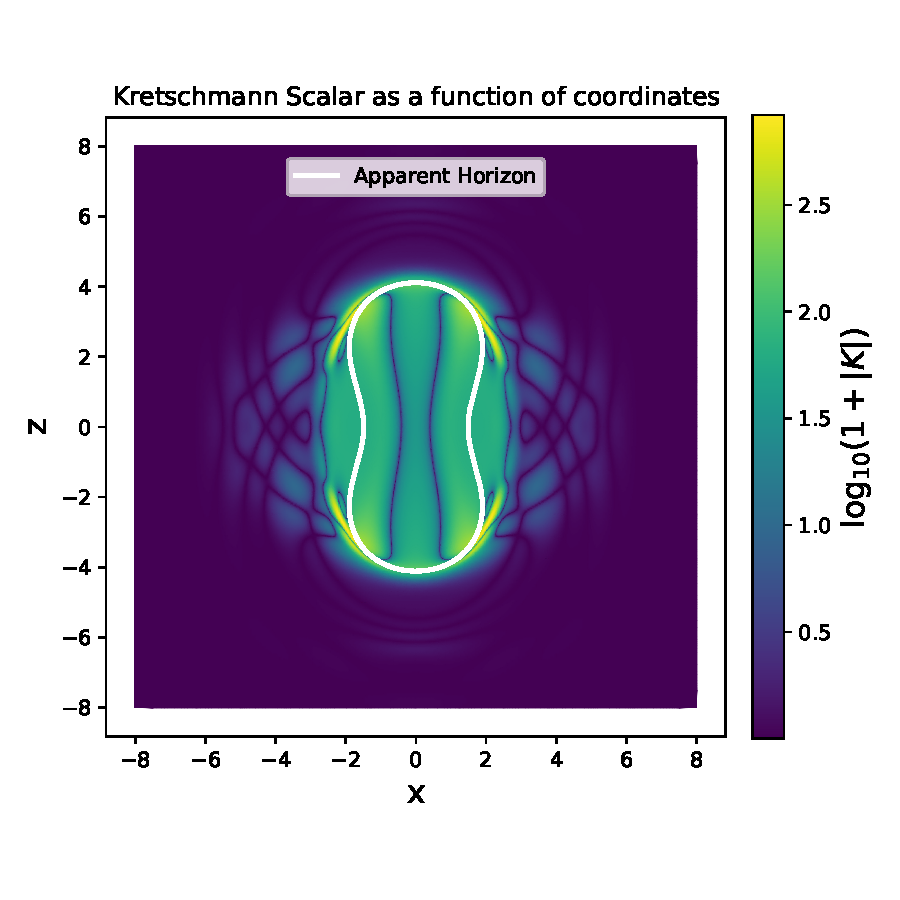
\includegraphics{notebooks/figure.pdf}
    \caption{}
\end{figure}

\subsubsection{Harmonic Horizon Marching Gauge}

Since GR has an intrinsic gauge freedom built into it, it will be reflected when we do simulations using NR as well. Hence we will have to choose a gauge but in the case of simulations they are chosen by the stability it confers to the simulations.

In \texttt{BAMPS}, the usual gauge that we use is HDWG (Harmonic Gauge). Here the evolution equations for the lapse becomes,

\[
\mathcal{L}_n \log \alpha = - (H_n +K)
\]

where $H_n$ is the free choosable function which only contains the metric and not its derivatives.

Inorder the push the lapse to 1 we add an extra term into the harmonic function in such a way that it adds a term $\eta_{hm}(\alpha-1)$ into the evolution equation for lapse

\[
\partial_t \alpha -\beta^i \partial_i \alpha= -\alpha^2(H_n + K)
\]

The extra term that in $H_n$ is $\eta_{hm} \alpha^{-2} (\alpha-1)$

\[
\partial_t \alpha -\beta^i \partial_i \alpha= -(\eta_{hm} (\alpha-1) + \alpha^2 K)
\]

So in $H_a$ an extra term of $-\eta_{hm} \alpha^{-2} (\alpha - 1) n_a$ is added

So New $H_0=.... + \eta_{hm} \alpha^{-1} (\alpha-1)$

\[
\partial_t H_0 = +\eta_{hm} \alpha^{-2} \partial_t \alpha
\]

\[
\partial_i H_0 = +\eta_{hm} \alpha^{-2} \partial_i \alpha
\]

\end{document}